\documentclass[10pt,twocolumn]{article}

\usepackage{times}
\usepackage{fullpage}
\usepackage{verbatim}
\usepackage{xcolor}
\usepackage[T1]{fontenc}
\usepackage{epsfig,endnotes,footnote}
\usepackage{graphicx,subfigure,array,multirow}
\usepackage{times,amsmath,amssymb}
\usepackage{enumitem}
\usepackage{booktabs}
\usepackage{xspace}
\usepackage{relsize}
\usepackage{hyphenat}
\usepackage{caption}
\captionsetup[figure]{labelfont=bf}


\setlength{\floatsep}{4pt} 
\setlength{\intextsep}{4pt}
\setlength{\textfloatsep}{4pt}

\usepackage{tabularx}

\graphicspath{{graphics/}}

\newcommand{\paragraphb}[1]{\vspace{0.05in}\noindent{\bf #1}\xspace}



\begin{document}

\title{\bf I/O Branch Bugs on Intermittent Systems}
\author{
Milijana Surbatovich
\and
Emily Ruppel
}
\date{}
\maketitle
\thispagestyle{empty}


\begin{abstract}
Batteryless energy harvesting devices are computing platforms that operate in
environments where batteries are not viable for energy storage.
Energy-harvesting devices operate intermittently, only as energy is available.
%
Prior work developed strategies for continuing long-running computations across
reboot cycles on energy harvesting devices. The strategies use a combination of
checkpointing volatile state and versioning non-volatile state to make
application code arbitrarily re-executable. However, prior work provides weak
guarantees for \emph{non-idempotent} operations such as reading from a sensor.
%
In the presence of control flow that is dependent on
non-idempotent operations, previous runtime systems allow updates from
uncommitted paths through the code to persist.
%
In this paper, we present a compiler pass that statically detects potentially
inconsistent writes to memory caused by non-idempotent operations and warns the
programmer.
%
We use the pass to analyze suites of embedded device code and found bugs caused
by inconsistent writes.


\end{abstract}

\section{Introduction}

Batteryless, energy harvesting devices are positioned to deliver an exciting new
class of applications enabled by maintenance free sensing and computing.
Batteryless devices harvest energy from their environments and store it in a
small buffer such as a capacitor rather than charging a battery.  The buffered
energy is used to operate a microprocessor as well as an array of peripherals
that gather and communicate data. As a result, these devices operate only
intermittently as energy is available.
%
Once all of the energy in the buffer has been used, the device powers down and
execution is terminated. Multiple systems have been developed to support long
running computations by continuing the execution across reboots. The
intermittent runtime systems developed in prior work use careful book-keeping of
program state to correctly perform the continuations  without custom hardware
~\cite{chain,dino,mementos,alpaca,mayfly,ratchet}.

When an execution is interrupted by a power failure, intermittent runtime
systems restore the most recent consistent state from a
checkpoint~\cite{mementos,ratchet}, or task boundary~\cite{chain,alpaca,dino} and
re-execute the segment of code that was interrupted.
%
All of these systems allow intermittently executed programs to make progress and
prevents persistent state from being corrupted by re-execution, however, their
guarantees in terms of sensor input are limited. Specifically, if \emph{control
flow} decisions are made based on non-idempotent operations, such as reading
input from a sensor, these systems allow updates from multiple branches to
persist.
%
This is a problem because re-executing the code and taking different branches on
each execution may result in writes to different variables, leaving the
previously written memory in an inconsistent state.
%
Bugs that can result from the partially written state are difficult for
programmers to diagnose because they require the programmer to reason about how
partial execution of different branches of control flow will affect the future
state of the program.
%
Instead, our project uses a compiler pass to identify control flow based on sensor input
and detect writes to non-volatile data that can leave memory in an inconsistent
state if repeated reads from the sensor produce different values.
%
% Is the following blurb still true?

In particular, our project focuses on refining the pass to
reduce the number of false positives the compiler generates by running the pass
on benchmarks used in intermittently powered devices. Initially, we intended to
use the MiBench suite of benchmarks for embedded devices, but we found that
MiBench applications primarily benchmark the computation performed by an
embedded device, not the device's handling of I/O. In the benchmarks we
investigated, sensor data are often represented as buffer of data that is
loaded once at the beginning of the application as opposed to pulled in
repeatedly as in a typical sensing application.



\section{Background}

...

\subsection{A discussion of non-idempotent behavior in intermittent programs}

In Figure \ref{fig:tax}, we present a flow chart of the taxonomy of non-idempotent behaviors and their potentially buggy consequences. 

\begin{figure}[ht]
\centering
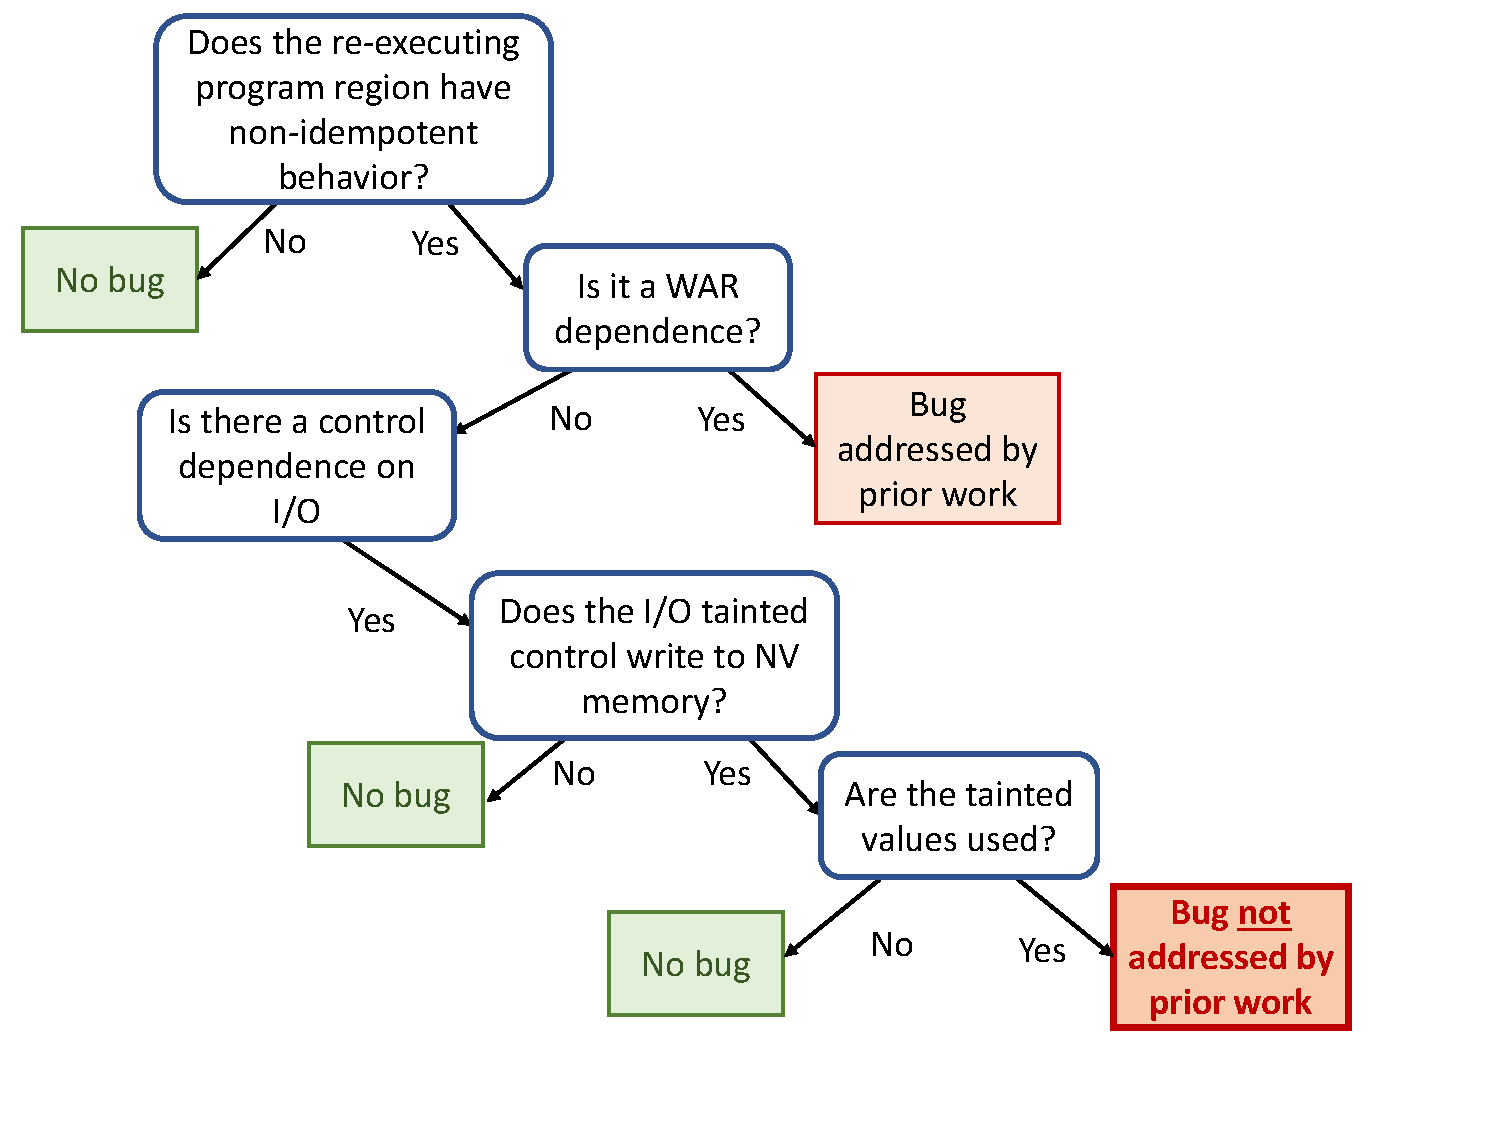
\includegraphics[width=1\columnwidth]{taxonomy.pdf}
\caption{Taxonomy of non-idempotent behavior and consequences}
\label{fig:tax}
\end{figure}
\paragraphb{Question 1: Does the program have non-idempotent behavior?}
Idempotent code can be re-executed arbitrarily without any changes to the
visible output~\cite{ratchet,dino}. Most new bugs introduced by computing under
intermittent power are due to memory inconsistencies caused by the unexpected
re-execution of code regions. If a program does not exhibit non-idempotent
behavior, it will not have any of the bugs we are studying.

\paragraphb{Questions 2 and 3: What is the cause of the non-idempotency?}
Non-idempotent behavior generally has two sources: write-after-read (anti)
dependencies and I/O operations.\footnote{Besides WAR dependencies and I/O,
there are some less common causes of non-idempotency, such as pointer-based
stack operations, as noted in prior work by Van Der Woude et al.
\cite{ratchet}.} Code re-execution after a WAR dependence creates direct
data-flow that did not exist in the original program, and I/O creates effects
that cannot be undone. Bugs off of WAR dependencies have been extensively
studied in prior work, and several runtime systems exist to fix them
\cite{ratchet, alpaca, dino}. While there could be other bugs
stemming from the use of irrevocable I/O operations, this paper specifically
explores memory inconsistencies stemming from branches that are control
dependent on non-idempotent input.

\paragraphb{Questions 4 and 5: When can an I/O dependent branch cause a bug?}
Not all I/O dependent branches necessarily lead to buggy behavior. To make
memory be in an inconsistent state, non-volatile variables must be written to on
at least one side of the branch, as they will still be visible to the program on
reboot. Furthermore, on a power fail and re-execution of the non-idempotent
region, such a tainted variable has to be the reaching definition for some use,
either in expected program execution or along the back-edge introduced by
re-executing. We discuss this further in Section [false positives]. If the
targets of the I/O dependent branch do write to non-volatile memory, however,
and there is some use of these tainted variables, this can cause bugs that have
not been addressed by prior work.
%		\item{Sometimes buggy behavior might only be exposed by re-orderings of
%		instructions during runtime. In such cases where the programmer %correctly
%		blocked the tainted variable from having any uses or wrote the exact same
%		non-volatile write set on both sides of the I/O branch, %compiler
%		optimizations might order the initializations on the wrong side of the reset
%		point [This would depend on the runtime system] or change %the order of the
%		non-volatile writes such that it is possible to write divergent sets on a
%		power fail. [Note: this needs to be written better.]} 

	


\section{System Overview}

The overarching algorithm is fixed-point - iterating through the functions, summarizing new information about the I/O flow, and iterating through functions again, until there is no new information to be gleaned. Psuedo-code is presented in Algorithm \ref{alg:fixedp}

\begin{algorithm}
\begin{algorithmic}
\Function{searchFunctions}{$Module M$} 
	\ForAll{Function func in M} 
		\State $workinglist \gets pair(func, NULL)$
	\EndFor
	
	\While{!workinglist.empty} 
		\State $currPair \gets workinglist.next$
		\State $sources \gets \Call{findTainted}{currPair}$ 
		\State $sinks \gets \Call{summarize}{sources}$
		\ForAll{taintedPair in sinks} 
			\State workinglist.add(taintedPair)
		\EndFor
	\EndWhile
\EndFunction
\\
\Function{findTainted}{pair(func, ioVal)} 
	\State $tainted \gets \Call{searchAnnotation}{func}$ 
	\State $visitlist \gets tainted$ 
	\While{!visitlist.empty}
		\State $current \gets visitlist.next$
		\State $result \gets \Call{traverseDependence}{current}$ 
		\ForAll{Instructions in result} 
			\If{instruction == BranchInst}
				\State \Call{check}{instruction, visitlist}
			\Else 
				\State Sources.add(instruction) 
			\EndIf
			
		\EndFor
	\EndWhile
	\State \Return{Sources}
\EndFunction
\\
\Function{traverseDependence}{tainted} 
	\ForAll{data dependencies of tainted} 
		\If{instruction == (BranchInst or Source)}
			\State result.add(instruction)
		\EndIf
		
	\EndFor
	
	\State \Return{result}
\EndFunction
\\
\Function{check}{branch, visitlist}
\ForAll{conditional target blocks on branch} 
	\ForAll{Instructions in block} 
		\If{instruction == store}
			\State bugReport[branch].add(instruction)
			\State visitList.add(instruction)
		\EndIf
	\EndFor
\EndFor
\EndFunction
\end{algorithmic}
\caption{Iterative, fixed point taint tracking. While the algorithm is not truly interprocedural, it tracks the data and control dependencies with the local function and summarizes how the taint flows out of the function. The summary information is used to add functions to the working list, until the entire I/O tainted flow has been explored}
\label{alg:fixedp}
\end{algorithm}
	
When the pass starts iterating, it doesn't know where the I/O enters the program, so all the functions are put in the working list, with a NULL I/O parameter--the I/O call is found internally, based on annotated information in the source code. Once the I/O source is found, the pass calls a function that traverses the data flow chain of the I/O instruction within the local function. In the chain, there are some instructions of interest: branches, which can lead to the bug of mismatched non-volatile write sets, and instructions that result in I/O tainted values flowing out of the current function that we're examining (an interprocedural flow {\bf source} ). 
	
Traversing the data flow primarily uses LLVM's built-in def-use chains. From the definition of the tainted variable, we follow the uses in a depth first search, adding on any new store instructions to the visit stack. 
From the traversal function call, we return the list of interesting instructions found to $findTainted$. If the instruction was a branch, the pass calls the $check$ function to examine the non-volatile write sets of the branch target blocks to see if there is the possibility for the bug. Additionally, any variables written to on the tainted branch are control-dependent on the I/O variable, so the pass adds any globals to the interprocedural source list and continues the local traversal with the newly tainted control dependent variables.

Once the pass finishes traversing the tainted flow within the local function, control returns back to $searchFunctions$ with the list of tainted sources of interprocedural flow. Based on the sources, the pass then calculates the corresponding sinks, as summarized in Table \ref{tab:interproc}.
	
If the tainted value was returned from some function F, the pass adds all the callers of F to the visit list, with the value where the return was stored as the tainted I/O value. Likewise if the tainted value was passed into a global, the pass finds the uses of the global, the parent function of those uses, and adds those to the visit list, with the global as the tainted value. If the I/O was used as an an argument in a call instruction, the pass searches for the callee function and the local version of the parameter. If I/O was stored into a pass-by-reference parameter, we find all the caller functions and their local value that the argument aliases to. 
	
The pass adds all these new function/tainted value pairs to the stack and continue to iterates, keeping track of what pairs have already been examined to prevent infinite looping. Eventually there will be no new information returned from the traversal function, and the pass has then finished examining all the functions to which the tainted I/O has spread. 

\begin{table*}[]
\centering
\begin{tabular}{|c|c|}
\toprule
Source & Sink\\ 
\midrule
Return value & Assignment in all caller functions \\
Global value & All uses of the global \\
Argument in a call instruction & Corresponding parameter in callee function \\
Pass-by-reference parameter & Corresponding argument in all caller functions \\
\bottomrule
\end{tabular}
\caption{Interprocedural flow sources and sinks}
\label{tab:interproc}
\end{table*}
	
\subsection{Checking the Write-sets}
Not all branches that are control dependent on non-idempotent I/O will necessarily cause a bug, as non-volatile variables must be written on at least one side of the branch. We check the conditionally executed target blocks for may-write instructions. We are not path-sensitive, so if a block has conditionals within it, we still add all the writes, even if they might actually be mutually exclusive, such as in an interior if-else branch. Once we have verified that there are non-volatile writes, we find that the results fall into three main categories: branches that have NV variables written on one side, branches that have \emph{different} NV variables written on both sides, and branches that have the \emph{same} variables written on both sides. The first two cases are the most likely to exhibit bugs. The first case can result in a block of statements that the programmer expects to be updated all together to only partially update, if execution fails in the middle of th writes and the other side of the branch is taken on re-execution. In the second case, potentially incompatible variables from both sides of the branch can be written, leading to a state inconsistent with any continuous execution of the program.  The third case, when the same variables are updated on both sides, is a little trickier. Originally, we did not report this as a bug, since any variables tainted by execution on one side of the branch will be overwritten if the other side is taken on re-execution. Control still has to reach this branch on re-execution, however, which it may not if the control path is altered on re-execution or if it is in a nested conditional. For this reason, we take a conservative approach and report all branches that write to NV variables, even if the write sets are the same. 

In the check function we also clear results that we know are false positives. Variables that are definitely overwritten on re-execution before any use of the tainted variable are effectively \textbf{sanitized}. While memory briefly exists in a state inconsistent with any continuous execution, it is never observed and thus does not actually effect program behavior.

To filter variables that must have been sanitized, we examine the instructions between the source of the taint and the relevant branch within the branch instruction's parent function. Since this is a local analysis, we consider the source of the taint as either coming from a particular instruction within the current function (such as the return value from a function or the original sensor read) or the top of the function, in the case of a tainted global or parameter. If an instruction between the source and branch writes to one of the variables in our branch write sets, we remove that value from the set. If no instructions remain in either set after filtering - all variables were santized - we remove the bug report for that branch. For the sake of time, we implement this filter as a simple function, but it could be interesting to make a more robust analysis pass.

\subsubsection{Pre-computing Non-volatile write-sets}

One challenge arises when an I/O dependent branch block itself calls a function, since any non-volatile writes within the called function should also be added to the branch clock write-set, adding a little context-sensitivity to our analysis.  To simplify handling the arbitrary complexity of control flow after leaving the target block (the called function could call another function, and so on), we pre-compute the {\bf may-write} sets of each function, using a bottom up examination of the call graph. Starting with the leaf functions, we track all non-volatile stores within a function, bubbling up those lists to the parent functions of a leaf. We repeat this procedure until we reach the root function. 
\section{Evaluation}
\section{Implications}

\begin{figure}[ht]
\centering
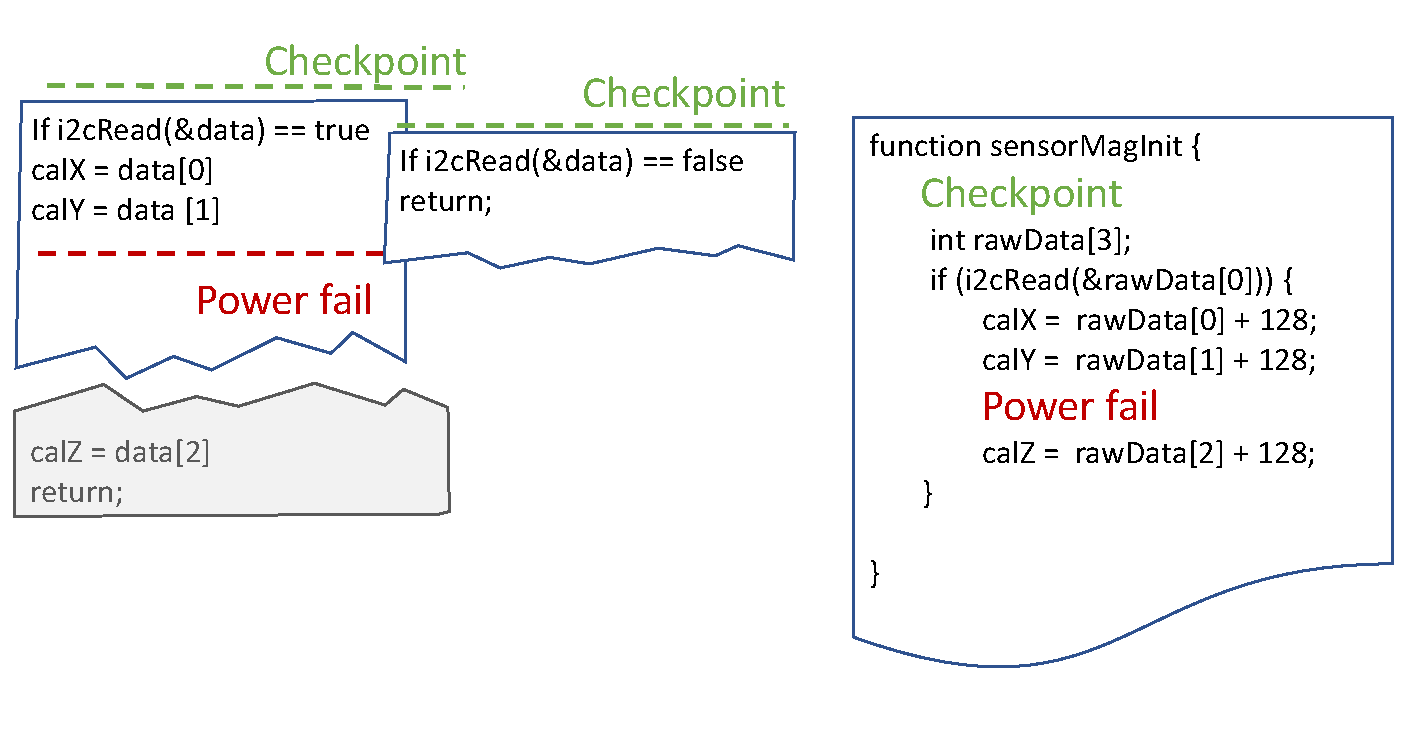
\includegraphics[width=1\columnwidth]{maginit_bug.pdf}
\caption{Bug in magnetometer initialization. Power failing while updating the calibration fields can cause the calibration data to become inconsistent, corrupting any future magnetometer reads that use the calibration.}
\label{fig:mag}
\end{figure}

\begin{figure}[ht]
\centering
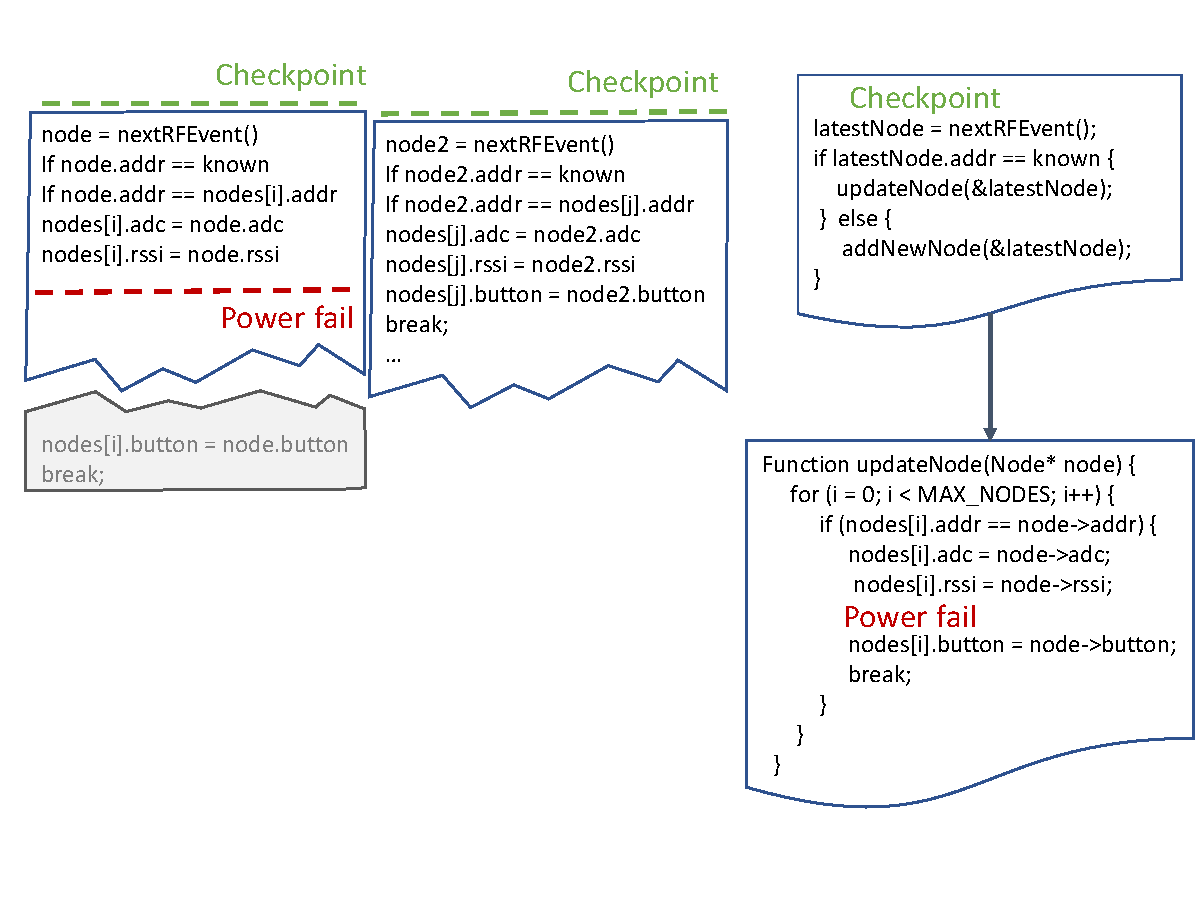
\includegraphics[width=1\columnwidth]{wsn_concentrator_bug.pdf}
\caption{Bug in WSN concentrator. Power failing while updating the node structure can cause the node list to become inconsistent, corrupting the payload ("button" field) or using out-of-date timing information}
\label{fig:wsn}
\end{figure}

\begin{figure}[ht]
\centering
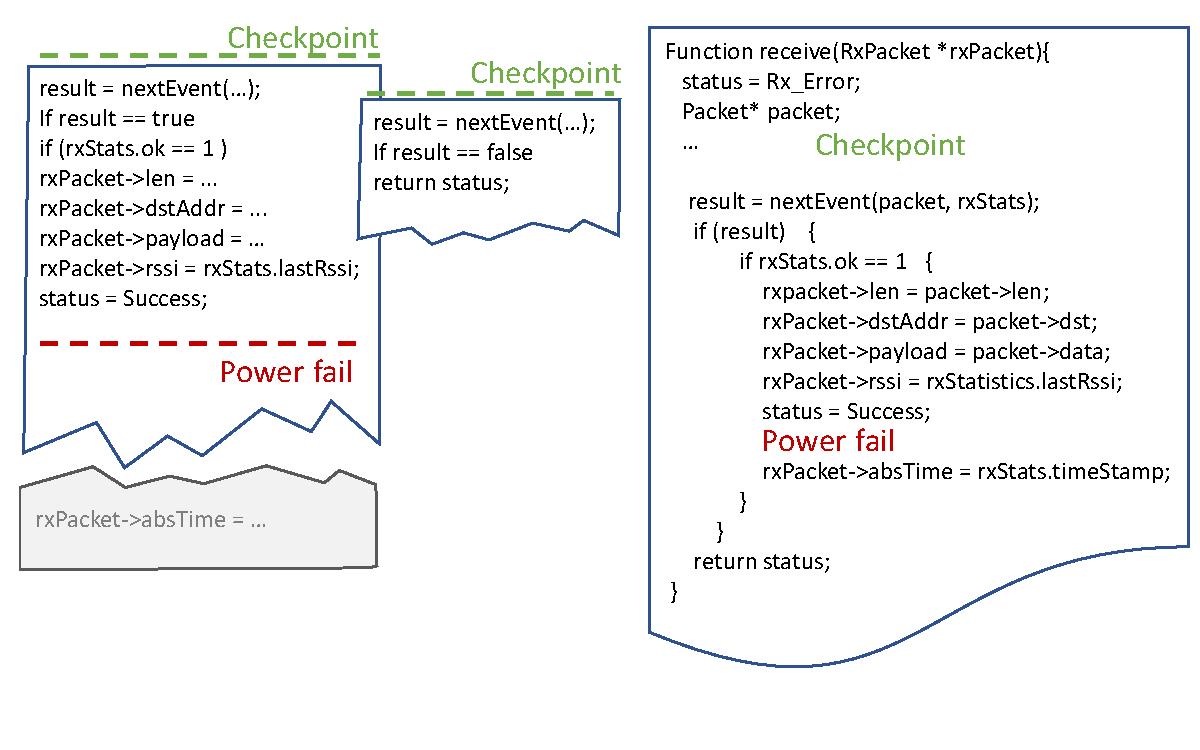
\includegraphics[width=1\columnwidth]{easylinkrx_bug.pdf}
\caption{Bug in RF EasyLink Receiver. Power failing before returning a correctly read packet can cause the status field to be set to success, even if the next event fails. The function will return an incorrect status value, potentially crashing the larger application.}
\label{fig:rf}
\end{figure}
\section{Surprises and Lessons Learned}
\section{Conclusion}


\bibliographystyle{abbrv} 
\bibliography{references}

\end{document}